\documentclass[11pt,a4paper]{article}
\usepackage[left=2cm,right=2cm,top=2cm,bottom=2cm]{geometry}
\usepackage{xcolor}
\usepackage{hyperref}
\usepackage{fontawesome5}
\usepackage{titlesec}
\usepackage{graphicx}
\usepackage{enumitem}
\usepackage{caption}
\usepackage{setspace}
\usepackage{tabularx}

% 줄간격 설정
\linespread{1.1}

\hypersetup{
    colorlinks=true,
    linkcolor=blue,
    filecolor=magenta,
    urlcolor=blue,
}

\titleformat{\section}
  {\Large\bfseries}
  {}{0em}
  {}
  [\titlerule]

\titleformat{\subsection}
  {\large\bfseries}
  {}{0em}
  {}

\setlist[itemize]{leftmargin=*, label=--, itemsep=0.3em}

\begin{document}

\begin{minipage}[t]{0.69\textwidth}
{\huge\bfseries 이력서}\\[0.8cm]
{\Large\bfseries 박상돈 박사}

\vspace{0.3cm}
박사 후 연구원\\
정보전자연구소, KAIST\\
대한민국 대전광역시 유성구 대학로 291, KAIST 34141\vspace{0.3cm}\\
\faEnvelope\ \href{mailto:johnsdpark@gmail.com}{johnsdpark@gmail.com} \hfill \faPhone\ +82-10-2523-3824 \\[0.2cm]
\faGlobe\ \href{https://sangdon-park.github.io/}{sangdon-park.github.io} \hfill \faLinkedin\ \href{https://www.linkedin.com/in/sangdon/}{linkedin.com/in/sangdon}
\end{minipage}%
\hfill
\begin{minipage}[t]{0.3\textwidth}
\vspace{-0.3cm}
\begin{flushright}
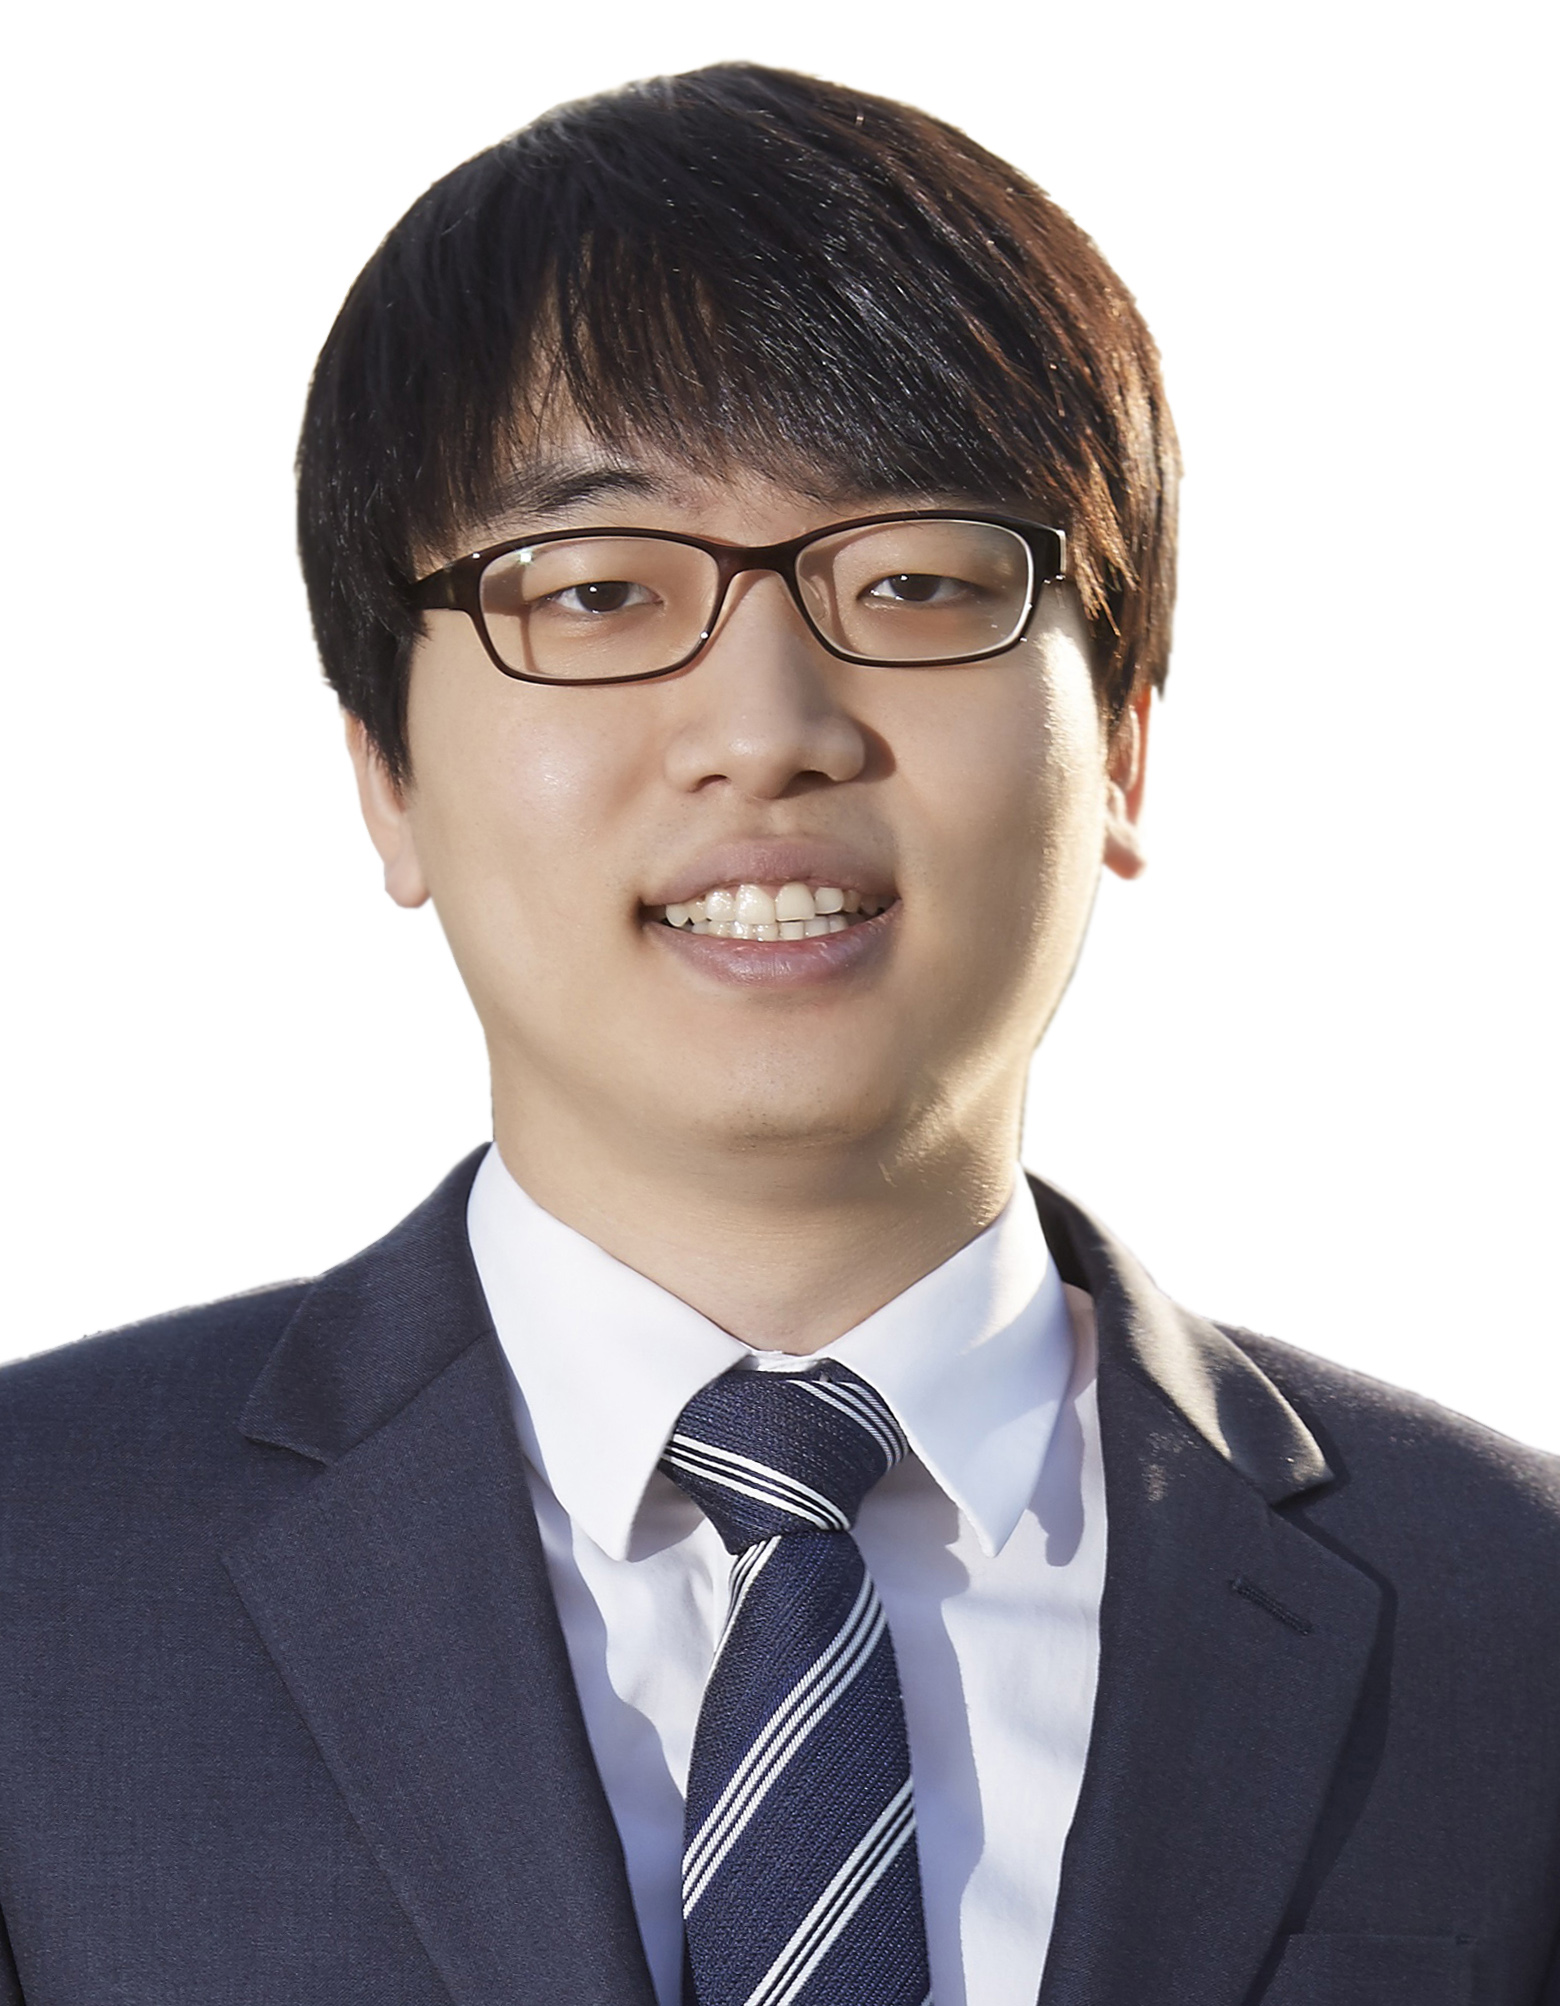
\includegraphics[width=0.7\textwidth]{Sangdon.jpg}
\end{flushright}
\end{minipage}

\vspace{0.3cm}
\linespread{1}
\section{경력}

\subsection*{AI 연구원/개발자 (예정), 세이베리 게임즈}
\textit{2024년 5월 -- 현재 (예정)} \hfill \textit{지도교수: 해당 없음}

\begin{itemize}
    \item LLM 기반 AI 캐릭터 및 인터랙티브 게임 시스템 연구 개발
    \item AI 기술을 활용한 게임 콘텐츠 제작 프로세스 혁신
\end{itemize}

\subsection*{박사 후 연구원, 정보전자연구소, KAIST}
\textit{2017년 8월 -- 현재} \hfill \textit{지도교수: 최준균}

\begin{itemize}
    \item 엣지 컴퓨팅, 에너지 거래, 데이터 시장 최적화 연구
    \item AI/LLM 기술 탐색 및 응용
\end{itemize}

\section{연구 개요}

박상돈 박사는 무선 네트워크, 스마트 그리드, 엣지 컴퓨팅 및 AI/LLM 응용 분야를 전문으로 하며, 최적화 및 자원 할당 메커니즘에 관한 전문 지식을 보유하고 있습니다. 2017년 KAIST에서 마이크로그리드의 에너지 거래 시스템 및 전력 시장에 초점을 맞춘 박사 학위를 취득했습니다. 2017년부터 KAIST에서 박사 후 연구원으로 활동하며 IoT, 분산 학습, 에너지 서비스 관련 주요 프로젝트에 참여했습니다. 2022년 3월, 엣지 컴퓨팅 연구의 책임 연구자로서 권위 있는 \textbf{세종과학펠로우십}(한국연구재단)을 수상하여 최대 5년 동안 연간 약 1억 2천만원을 지원받고 있습니다.

지난 8개월 동안 박상돈 박사는 LLM 응용(ChatGPT, Claude, Gemini)을 집중적으로 탐구하여, 4년 프로젝트로 여겨졌던 \textbf{엣지 컴퓨팅 GUI 시뮬레이터}를 단 한 달 만에 구현했습니다. 그의 \textbf{AI 캐릭터 대화} 프로젝트는 단순한 대화를 넘어 자연스러운 캐릭터 상호작용을 구현하는 탁월한 능력을 보여주며, 게임 개발에 새로운 가능성을 열었습니다. 그는 AI 코딩 도구를 효과적으로 활용하여 개발 생산성과 빠른 프로토타이핑을 향상시킵니다.

최근 AI 기술 관련 연구를 바탕으로 박상돈 박사는 2024년 5월에 \textbf{세이베리 게임즈}에 합류하여 AI 기반 인터랙티브 경험 연구에 참여할 예정이며, 3억원 규모의 \textbf{AI 게임 개발 프로젝트}를 확보했습니다. 현재 그의 연구 관심사는 LLM 기반 시스템 설계, AI 캐릭터 및 인터랙티브 시스템, AI 기반 시뮬레이션 및 최적화, AI 도구를 통한 개발 생산성 향상 등입니다. 그는 최첨단 AI 방법론과 함께 수학적 이론을 사용하여 시스템을 엄격하게 모델링하고 있습니다.

\section{학력}

\begin{tabular}{p{14cm}r}
\textbf{KAIST 전기 및 전자공학부 박사} & 2013--2017 \\
\\
\textit{논문:} Dynamic Energy Trading Scheme for Future Smart Grid & \\
\textit{지도교수:} 최준균 교수 (미디어 네트워크 연구실) & \\
\textit{연구 분야:} 무선 통신, 스마트 그리드, 최적화, 게임 이론, 에너지 빅데이터 & \\
\\
\textbf{KAIST 수리과학과 석사} & 2011--2013 \\
\\
\textit{논문:} Throughput Performance Analysis of Optimal Random Access Policies for & \\
Cognitive Radio Networks & \\
\textit{지도교수:} 황강욱 교수 (차세대 통신 네트워크 연구실) & \\
\textit{연구 분야:} 확률 과정, 대기 이론, 확률론, 무선 통신 & \\
\\
\textbf{KAIST 수리과학과 학사} & 2006--2011 \\
\end{tabular}

\section{연구비 수주}

\begin{tabular}{p{14cm}r}
\textbf{세종과학펠로우십 (국내트랙), 한국연구재단} & 2022--현재 \\
연간 1억 2천만원, 3+2년 지원, 현재 4년차 & \\
\\
\textbf{기초연구사업, 한국연구재단} & 2018--2022 \\
2억원 (4년) & \\
``스마트 계약을 이용한 학습 기반 에너지 거래 블록체인 기술'' & \\
주로 젊은 교수를 지원하는 이 사업에서 극히 예외적인 사례임 & \\
\\
\textbf{BK21 플러스 프로그램, 한국연구재단} & 2017--2019 \\
4천 5백만원 (1.5년) & \\
\end{tabular}

\section{논문}

\subsection{대표 논문 (* 교신저자, † 제1저자)}

\begin{enumerate}[label={[{\arabic*}]}, leftmargin=*, itemsep=0.3em]
\item \textbf{Sangdon Park†}; Joohyung Lee; Sohee Bae; Ganguk Hwang; Jun Kyun Choi, ``Contribution-Based Energy-Trading Mechanism in Microgrids for Future Smart Grid: A Game Theoretic Approach,'' \textit{IEEE Transactions on Industrial Electronics}, vol. 63, no. 7, pp. 4255--4265, 2016. (인용수: 243)

\item Hyeontaek Oh; \textbf{Sangdon Park*}; Gyu Myoung Lee; Hwanjo Heo; Jun Kyun Choi, ``Personal Data Trading Scheme for Data Brokers in IoT Data Marketplaces,'' \textit{IEEE Access}, vol. 7, pp. 40120--40132, 2019. (인용수: 90)

\item Beomhan Baek; Joohyung Lee; Yuyang Peng; \textbf{Sangdon Park*}, ``Three Dynamic Pricing Schemes for Resource Allocation of Edge Computing for IoT Environment,'' \textit{IEEE Internet of Things Journal}, vol. 7, no. 5, pp. 4292--4303, 2020. (인용수: 89)

\item Hyeontaek Oh; \textbf{Sangdon Park*}; Gyu Myoung Lee; Jun Kyun Choi; Sungkee Noh, ``Competitive Data Trading Model with Privacy Valuation for Multiple Stakeholders in IoT Data Markets,'' \textit{IEEE Internet of Things Journal}, vol. 7, no. 4, pp. 3623--3639, 2020. (인용수: 77)

\item Seong-Hwan Kim; \textbf{Sangdon Park*}; Min Chen; Chan-Hyun Youn, ``An Optimal Pricing Scheme for the Energy-Efficient Mobile Edge Computation Offloading with OFDMA,'' \textit{IEEE Communications Letters}, vol. 22, no. 9, pp. 1922--1925, 2018. (인용수: 71)

\item Hyeonseok Seo; Hyeontaek Oh; Jun Kyun Choi; \textbf{Sangdon Park*}, ``Differential Pricing-Based Task Offloading for Delay-Sensitive IoT Applications in Mobile Edge Computing System,'' \textit{IEEE Internet of Things Journal}, vol. 9, no. 19, pp. 19116--19131, 2022. (인용수: 26)
\end{enumerate}

\subsection{국제 저널}

\begin{enumerate}[label={[{\arabic*}]}, leftmargin=*, itemsep=0.3em]

% 2024
\item \textbf{Sangdon Park}; Sohee Bae; Joohyung Lee; Youngchul Sung, ``Real-Time Dynamic Pricing for Edge Computing Services: A Market Perspective,'' \textit{IEEE Access}, vol. 12, pp. 134754--134769, 2024.

\item Mohammed, A.; Lee, J.; \textbf{Sangdon Park*}, ``Dynamic Bandwidth Slicing in Passive Optical Networks to Empower Federated Learning,'' \textit{Sensors}, vol. 24, no. 15, 2024.

% 2022
\item Hyeonseok Seo; Hyeontaek Oh; Jun Kyun Choi; \textbf{Sangdon Park*}, ``Differential Pricing-Based Task Offloading for Delay-Sensitive IoT Applications in Mobile Edge Computing System,'' \textit{IEEE Internet of Things Journal}, vol. 9, no. 19, pp. 19116--19131, 2022.

\item Jaeseob Han; Gyeong Ho Lee; \textbf{Sangdon Park*}; Jun Kyun Choi, ``Joint Subcarrier and Transmission Power Allocation in OFDMA-Based WPT System for Mobile-Edge Computing in IoT Environment,'' \textit{IEEE Internet of Things Journal}, vol. 9, no. 16, pp. 15039--15052, 2022.

\item Yue Zang; Yuyang Peng; \textbf{Sangdon Park}; Han Hai; Fawaz Al-Hazemi; Mohammad Meraj Mirza, ``A Novel Cooperative Transmission Scheme in UAV-Assisted Wireless Sensor Networks,'' \textit{Electronics}, vol. 11, no. 4, 2022.

\item Jangkyum Kim; Joohyung Lee; \textbf{Sangdon Park}; Jun Kyun Choi, ``Power Scheduling Scheme for a Charging Facility Considering the Satisfaction of Electric Vehicle Users,'' \textit{IEEE Access}, vol. 10, pp. 25153--25164, 2022.

% 2021
\item Jaeseob Han; Gyeong Ho Lee; \textbf{Sangdon Park*}; Joohyung Lee; Jun Kyun Choi, ``A Multivariate-Time-Series-Prediction-Based Adaptive Data Transmission Period Control Algorithm for IoT Networks,'' \textit{IEEE Internet of Things Journal}, vol. 9, no. 1, pp. 419--436, 2021.

\item Jinhwan Jeon; Yoonjin Hwang; Yongseop Jeong; \textbf{Sangdon Park}; In So Kweon; Seibum B. Choi, ``Lane Detection Aided Online Dead Reckoning for GNSS Denied Environments,'' \textit{Sensors}, vol. 21, no. 20, 2021.

\item Hyeontaek Oh; \textbf{Sangdon Park*}; Jun Kyun Choi; Sungkee Noh, ``Deposit Decision Model for Data Brokers in Distributed Personal Data Markets Using Blockchain,'' \textit{IEEE Access}, vol. 9, pp. 114715--114726, 2021.

% 2020
\item Beomhan Baek; Joohyung Lee; Yuyang Peng; \textbf{Sangdon Park*}, ``Three Dynamic Pricing Schemes for Resource Allocation of Edge Computing for IoT Environment,'' \textit{IEEE Internet of Things Journal}, vol. 7, no. 5, pp. 4292--4303, 2020.

\item Hyeontaek Oh; \textbf{Sangdon Park*}; Gyu Myoung Lee; Jun Kyun Choi; Sungkee Noh, ``Competitive Data Trading Model with Privacy Valuation for Multiple Stakeholders in IoT Data Markets,'' \textit{IEEE Internet of Things Journal}, vol. 7, no. 4, pp. 3623--3639, 2020.

\item Gyohun Jeong; \textbf{Sangdon Park*}; Ganguk Hwang, ``Time Series Forecasting Based Day-Ahead Energy Trading in Microgrids: Mathematical Analysis and Simulation,'' \textit{IEEE Access}, vol. 8, pp. 63885--63900, 2020.

% 2019
\item Jangkyum Kim; Joohyung Lee; \textbf{Sangdon Park}; Jun Kyun Choi, ``Battery-Wear-Model-Based Energy Trading in Electric Vehicles: A Naive Auction Model and a Market Analysis,'' \textit{IEEE Transactions on Industrial Informatics}, vol. 15, no. 7, pp. 4140--4151, 2019.

\item \textbf{Sangdon Park}; Ganguk Hwang; Jun Kyun Choi, ``Optimal Throughput Analysis of Multiple Channel Access in Cognitive Radio Networks,'' \textit{Annals of Operations Research}, vol. 277, no. 2, pp. 345--370, 2019.

\item Yuyang Peng; Jun Li; \textbf{Sangdon Park*}; Konglin Zhu; Mohammad Mehedi Hassan; Ahmed Alsanad, ``Energy-Efficient Cooperative Transmission for Intelligent Transportation Systems,'' \textit{Future Generation Computer Systems}, vol. 94, pp. 634--640, 2019.

\item Jaewon Ahn; Joohyung Lee; \textbf{Sangdon Park}; Hong-Shik Park, ``Power Efficient Clustering Scheme for 5G Mobile Edge Computing Environment,'' \textit{Mobile Networks and Applications}, vol. 24, no. 2, pp. 643--652, 2019.

\item Hyeontaek Oh; \textbf{Sangdon Park*}; Gyu Myoung Lee; Hwanjo Heo; Jun Kyun Choi, ``Personal Data Trading Scheme for Data Brokers in IoT Data Marketplaces,'' \textit{IEEE Access}, vol. 7, pp. 40120--40132, 2019.

\item Sohee Bae; \textbf{Sangdon Park*}, ``Comparison Between Seller and Buyer Pricing Systems for Energy Trading in Microgrids,'' \textit{IEEE Access}, vol. 7, pp. 54084--54096, 2019.

% 2018
\item Nakyoung Kim; \textbf{Sangdon Park*}; Joohyung Lee; Jun Kyun Choi, ``Load Profile Extraction by Mean-Shift Clustering with Sample Pearson Correlation Coefficient Distance,'' \textit{Energies}, vol. 11, no. 9, 2018.

\item Seong-Hwan Kim; \textbf{Sangdon Park*}; Min Chen; Chan-Hyun Youn, ``An Optimal Pricing Scheme for the Energy-Efficient Mobile Edge Computation Offloading with OFDMA,'' \textit{IEEE Communications Letters}, vol. 22, no. 9, pp. 1922--1925, 2018.

\item Busik Jang; \textbf{Sangdon Park*}; Joohyung Lee; Sang-Geun Hahn, ``Three Hierarchical Levels of Big-Data Market Model Over Multiple Data Sources for Internet of Things,'' \textit{IEEE Access}, vol. 6, pp. 31269--31280, 2018.

\item Sanghong Ahn; Joohyung Lee; \textbf{Sangdon Park*}; S.H. Shah Newaz; Jun Kyun Choi, ``Competitive Partial Computation Offloading for Maximizing Energy Efficiency in Mobile Cloud Computing,'' \textit{IEEE Access}, vol. 6, pp. 899--912, 2018.

% 2017
\item \textbf{Sangdon Park}; Joohyung Lee; Ganguk Hwang; Jun Kyun Choi, ``Event-Driven Energy Trading System in Microgrids: Aperiodic Market Model Analysis with a Game Theoretic Approach,'' \textit{IEEE Access}, vol. 5, pp. 26291--26302, 2017.

\item Minkyung Kim; \textbf{Sangdon Park}; Joohyung Lee; Yongjae Joo; Jun Kyun Choi, ``Learning-Based Adaptive Imputation Method with kNN Algorithm for Missing Power Data,'' \textit{Energies}, vol. 10, no. 10, 2017.

% 2016
\item \textbf{Sangdon Park}; Joohyung Lee; Sohee Bae; Ganguk Hwang; Jun Kyun Choi, ``Contribution-Based Energy-Trading Mechanism in Microgrids for Future Smart Grid: A Game Theoretic Approach,'' \textit{IEEE Transactions on Industrial Electronics}, vol. 63, no. 7, pp. 4255--4265, 2016.
\end{enumerate}

\subsection{국제 학술대회}

\begin{enumerate}[label={[{\arabic*}]}, leftmargin=*, itemsep=0.3em]

% 2021
\item J Lee; M Kim; \textbf{Sangdon Park}; J.K. Choi; Y Hwang, ``Driver Identification for Different Road Shapes Using Vehicle IoT Sensing Data,'' in \textit{Proceedings of the 2021 IEEE International Conference on Consumer Electronics (ICCE)}, Las Vegas, NV, USA, January 10--12, 2021.

% 2018
\item J Han; \textbf{Sangdon Park}; G.H. Lee; M Kim; H Seo; J.K. Choi, ``Energy Trading in Wireless Power Transmission System Considering Nonlinear Rectifier,'' in \textit{Proceedings of the 2018 IEEE 7th Global Conference on Consumer Electronics (GCCE)}, Nara, Japan, October 9--12, 2018.

\item Eunju Yang; Seong Hwan Kim; TaeWoo Kim; Min Su Jeon; \textbf{Sangdon Park}; Chan-Hyun Youn, ``An Adaptive Batch-Orchestration Algorithm for the Heterogeneous GPU Cluster Environment in Distributed Deep Learning System,'' in \textit{Proceedings of the 2018 IEEE International Conference on Big Data and Smart Computing (BigComp)}, Shanghai, China, January 15--17, 2018.

\item Minkyung Kim; \textbf{Sangdon Park}; Kireem Han; Nakyoung Kim; Jun Kyun Choi, ``Dynamics of Electricity Consumers for Classifying Power Consumption Data Using PCA,'' in \textit{Proceedings of the 2018 IEEE International Conference on Big Data and Smart Computing (BigComp)}, Shanghai, China, January 15--17, 2018.

% 2017
\item \textbf{Sangdon Park}; Justin Weimer; Insup Lee, ``Resilient Linear Classification: An Approach to Deal with Attacks on Training Data,'' in \textit{Proceedings of the 8th ACM/IEEE International Conference on Cyber-Physical Systems (ICCPS)}, Pittsburgh, PA, USA, April 18--21, 2017.

% 2016
\item \textbf{Sangdon Park}; Jae Deok Kim; Ganguk Hwang; Jun Kyun Choi, ``Joint Optimal Access and Sensing Policy on Distributed Cognitive Radio Networks with Channel Aggregation,'' in \textit{Proceedings of the 2016 Eighth International Conference on Ubiquitous and Future Networks (ICUFN)}, Vienna, Austria, July 5--8, 2016.

\item Hyeontaek Oh; S.H. Shah Newaz; \textbf{Sangdon Park}; Jun Kyun Choi, ``Maximizing Energy Efficiency in Off-Peak Hours: A Novel Sleep Scheme for WLAN Access Points,'' in \textit{Proceedings of the 2016 IEEE/IFIP Network Operations and Management Symposium (NOMS)}, Istanbul, Turkey, April 25--29, 2016.

\item \textbf{Sangdon Park}; Ganguk Hwang; Jun Kyun Choi, ``Optimal Throughput Analysis of Random Access Policies for Cognitive Radio Networks with Multiple Channel Access,'' in \textit{Proceedings of the 11th International Conference on Queueing Theory and Network Applications (QTNA)}, Wellington, New Zealand, December 13--15, 2016.

% 2013
\item Seonghwa Yun; Kyeongmin Lee; \textbf{Sangdon Park}; Jun Kyun Choi, ``Energy Efficient Relay Selection Scheme with DRX Mechanism in 3GPP LTE Network,'' in \textit{Proceedings of the 2013 International Conference on ICT Convergence (ICTC)}, Jeju Island, South Korea, October 14--16, 2013.
\end{enumerate}

\section{표준화 활동}

\begin{tabularx}{\textwidth}{X}
\textbf{국제전기통신연합 전기통신 표준화 부문 (ITU-T) 표준} \\[0.2cm]
대한민국 대표, ITU-T SG13 및 SG5 \hfill \textit{2013년 6월 -- 2014년 11월}\\
\\[0.3cm]
\textbf{ITU-T SG13 보고관 회의} \hfill \textit{2013년 6월, 제네바, 스위스}
\\[0.2cm]
\textbf{Sangdon Park}; Seung Hyun Jeon; Jun Kyun Choi; Jeong Yun Kim, ``Consideration of classification of sleep mode control on network equipment,'' SG13RGM-C-06 \\[-0.2cm]
\\
Seung Hyun Jeon; \textbf{Sangdon Park}; Jun Kyun Choi, ``Revised draft Recommendation Y.energyMRM for requesting the consent,'' SG13RGM-C-04 \\[-0.2cm]
\\
Seung Hyun Jeon; \textbf{Sangdon Park}; Jun Kyun Choi; Jeong Yun Kim, ``Consideration of classification for CPU power consumption on network equipment,'' SG13RGM-C-05 \\
\\[0.3cm]
\textbf{ITU-T SG13 회의} \hfill \textit{2013년 11월, 캄팔라, 우간다} \\[0.2cm]
\textbf{Sangdon Park}; Gyu Myoung Lee; Jun Kyun Choi, ``Proposal of the new draft recommendation Y.energyECN (Energy efficiency class of network equipment),'' COM13-C401-E \\
\\[0.3cm]
\textbf{ITU-T SG13 보고관 회의} \hfill \textit{2014년 2월, 제네바, 스위스} \\[0.2cm]
\textbf{Sangdon Park}; Jaewon Ahn; Jun Kyun Choi; Gyu Myoung Lee, ``A proposal for definitions of energy efficiency class of network equipment,'' SG13RGM-C-94 \\[-0.2cm]
\\
\textbf{Sangdon Park}; Jaewon Ahn; Jun Kyun Choi; Gyu Myoung Lee, ``Revised texts for a main chapter of draft recommendation,'' SG13RGM-C-75 \\[-0.2cm]
\\
\textbf{Sangdon Park}; Jun Kyun Choi; Gyu Myoung Lee, ``A proposal for definitions of energy efficiency class of network equipment,'' SG13RGM-C-75 \\
\end{tabularx}

\section{교육 활동}

\begin{tabular}{p{14cm}r}
\textbf{설계 조교} & 2014년 봄학기 \\
``전자설계 및 실험 개론'', KAIST 전기 및 전자공학부 & \\
\\
\textbf{상담 조교} & 2013년 가을학기 \\
KAIST 전기 및 전자공학부 & \\
\\
\textbf{교육 조교} & 2012년 가을학기 \\
미적분학 II, KAIST 수리과학과 & \\
\\
\textbf{교육 조교} & 2012년 봄학기 \\
미적분학 I, KAIST 수리과학과 & \\
\\
\textbf{교육 조교} & 2011년 가을학기 \\
선형대수학 개론, KAIST 수리과학과 & \\
확률 및 통계, KAIST 수리과학과 & \\
\end{tabular}

\end{document}
